\chapter{System Development} \label{system_development}

This section will present the development and workflow of the system. 
As previously mentioned, the next step was to expand the defined DSL, and to use attributes as a form of calculation. 
Most of the productions were expanded, allowing for certain calculations to be injected over the tree.

\section{Meta-Grammar}

With the grammar divided into 3 main parts (STRUCTURE, ERRORS, INPUT), different types of calculations occur at different sections. The STRUCTURE and ERRORS blocks are written in a single file (by the teacher) which is then joined 
with the INPUT block (written by the student). The process starts with searching for the teacher and student specification, and then compiling the program using a meta-grammar based processor. A new processor is generated to be 
used by the student to verify if his sentences are correctly following the structure defined by the teacher.

Within the grammar itself, the first rule
\newpage

%\begin{center}
%\begin{minipage}{11cm}
%\begin{Verbatim}[frame=single, framesep=2mm, fontsize=\small]
%determinante returns[Integer genero, Integer numero]
%    : ('A' | 'a')
%        { $genero = FEMININO; $numero = SINGULAR; }
%    | ('O' | 'o')
%        { $genero = MASCULINO; $numero = SINGULAR; }
%    | ('As' | 'as')
%        { $genero = FEMININO; $numero = PLURAL; }
%    | ('Os' | 'os')
%        { $genero = MASCULINO; $numero = PLURAL; }
%
%    (...)
%;
%\end{Verbatim}
%\end{minipage}
%\end{center}

\begin{center}
\begin{minipage}{11cm}
\begin{lstlisting}[language=java, basicstyle=\small, label={lst:processor}, caption=Processor rule from the meta-grammar]
processor
@init {
    /* Main data structure. */
    List<RoseTree> struct = new ArrayList<>();

    (...)
}
    : structure[struct]
      errors[struct]
      input[struct]
    {
        (...)
    }
\end{lstlisting}
\end{minipage}
\end{center}

\noindent starts by initializing the main data structure. This structure is responsible for storing all the information that is being parsed from the file given as input (the meta-language file). 

When choosing the correct structure to store all the important data, the first \/\*approach\*\/ taken was to store all components in a single Map, with each name of a component
matching their respective value. The problem with this approach, which was identified right away, was that is possible to exist two or more components with the same exact
name, causing a conflict within the Map. Furthermore, components have different information associated, like attributes, and it would be better if it is all in the same
place - this created the need for a Component class.

The Component class would store the name of the component, a possible value and a Map that associated each attribute with some value. The components would all be stored
within a List.
\newpage

\begin{center}
\begin{minipage}{10cm}
\begin{lstlisting}[language=java, basicstyle=\small, label={lst:component_class}, caption=Component class]
@members {
    class Component {
        String name;
        String lexical_part;
        Map<String, String> attributes;
    }

    /* Main data structure. */
    List<Component> struct;
}
\end{lstlisting}
\end{minipage}
\end{center}

The problem with this solution is that it does not follow any particular order (in this case, the STRUCTURE order), which can be very useful when validating the students
input, checking if it obeys to the structure previously defined.

The structure of the sentence takes a form of a tree, so that would be the correct way to store the information and maintain order. As each node could have less or more 
than two children, a binary tree was not the way to go. The idea was to build a Graph structure that used a mapped each node to a list of nodes.

\begin{center}
\begin{minipage}{11cm}
\begin{lstlisting}[language=java, basicstyle=\small, label={lst:graph_class}, caption=Graph class]
@members {
    class Graph
    {
        Map<Component, List<Component>> map;
    }
}
\end{lstlisting}
\end{minipage}
\end{center}

Although this could maintaing the order, the initial problem remainded. We could have components with the same exact properties, and this would cause conflict between
edges, and not create a new node when it was supposed to.

The principle of having a tree as the main data structure falls into the need of maintaining a valid path. For example, if the teacher says that the structure will have a component \emph{\textbf{A}}, and this component has two children, \emph{\textbf{B}} and \emph{\textbf{C}}, then the paths \emph{\textbf{A$\rightarrow$B}} and \emph{\textbf{A$\rightarrow$C}} should be stored. In this particular problem, it is required to have a tree that within each node has a list of children with an arbitrary size of \emph{\textbf{N}}.

Some backtracking was made to come up with an ideal solution. The prerequisites were that order needed to be maintained and each node (component) had an arbitrary number
of \emph{\textbf{N}} children. The previously created Component class would store all its values and a list of new components (children), creating a path between 
the parent component and said children. This type of structure is denominated as Rose Tree, which is a prevelant structure in the functional programming community. 
It is a multi-way tree, with an unbounded number of branches per node. This way, all the prerequisites would be matched, and all the information correctly stored. 

\begin{center}
\begin{minipage}{9cm}
\begin{lstlisting}[language=java, basicstyle=\small, label={lst:rosetree_class}, caption=RoseTree class]
class RoseTree {
    String value;
    boolean required;
    Map<String, String> attributes;
    List<String> lexical_part;
    List<RoseTree> children;

    (...)
}
\end{lstlisting}
\end{minipage}
\end{center}

When in the main production (\emph{processor}), a list of \emph{Rose Trees} is initialized, with each tree of the list corresponding to the main components of the sentence. This structure would travel along the parsing tree, to first be populated with information and then serving as the main source of validation and checking.

On the first block (STRUCTURE) there are not many calculations happening within the productions. 
The main task is to simply validate the syntax and extract data to be stored in the \emph{Rose Tree}. 
For each node, it is stored the name of the component, if it is required to be declared or not, a group of attributes (could be non-existent), 
a lexical part (if it is the case), and finally a list of nodes, referred as the children.

After the parsing of the structure, there are a list of conditions named ERRORS that need to be validated and converted into \emph{Java} syntax - this conversion would then be injected on the main rule of the generated grammar. These logical expressions are based on the attributes of each component and their relations. For example, if the teacher says that a component \emph{\textbf{A}} has an attribute named \emph{\textbf{a}}, and this attribute is required to have value \emph{\textbf{x}}, if the student assigns it a value of \emph{\textbf{z}}, then an error should appear. All these conditions can be combined with the logical operands ``AND'' or ``OR''. The way that is parsed is based on the path specified by the teacher when accessing the attribute. Using the example before, a component \emph{\textbf{A}} with a child \emph{\textbf{B}}, with \emph{\textbf{B}} having a attribute \emph{\textbf{x}}, in order to access it the syntax should be

A.B -\textgreater x

\noindent as the full path is required. This is done in order to calculate the correct path and avoid ambiguity between attributes. Over the parsing of these rules, the path is being validated, and in case of any error, the user is notified.

Finally, the last block corresponds to the input that was written by the student. 
The goal is to validate the components that were defined, and match them with the structure created by the teacher. 
Again, the RoseTree was used as a way to check if the student’s components and paths were valid. 
The task of the student was to ``parse'' his sentence and divide it by components, identifying the lexical segments and storing them within a node of the \emph{Rose Tree}. 
At last, the main rule of the Meta-Grammar makes use of a generator to generate all the rules for the Specific Natural Language Grammar. 
Within this generator, the various \emph{Rose Tree's} are passed as an argument and then traversed recursively.
% In the case of any error, the user is informed of where the error happened but also in which component. 
% Furthermore, when parsing attributes and their respective values, if the student defines two attributes with the same name, but with different values, 
% a warning is raised to inform the user that the value that was considered was the last one to be recognized.

\section{Meta-Language Processor}

In order to simplify the usage of the Meta-Grammar, and as the grammar itself made use of auxiliar \emph{Java} classes, all of that was combined into a \emph{JAR} file.
Having this type of package would allow for a more flexible integration with any component.
The Meta-Language Processor, which was created by providing the Meta-Grammar file to ANTLR, could now be used with the \emph{JAR} file, 
providing as input the Meta-Language Specification. 

Using the command line, the instruction:
\begin{Verbatim}
	java -jar lib/MetaGrammar.jar input/meta-lang
\end{Verbatim}
\noindent tries to generate the Specific Natural Language Grammar, based on the input provided. In case of any error, the grammar would not be generated.

\begin{figure}[h]
    \centering
    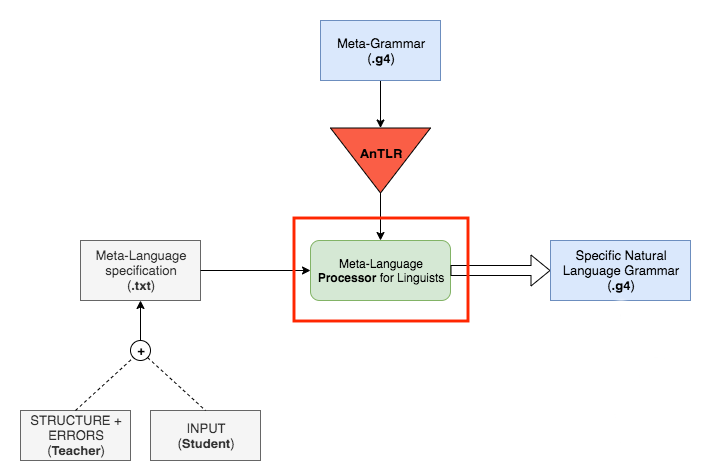
\includegraphics[width=10cm]{images/system_meta_processor.png}
    \caption{Excerpt of the system architecture.}
    \label{fig:system_architecture}
\end{figure}

\section{Sentence Validator}

If no errors occur in the previous step, we should now have a file named ``Grammar.g4" that corresponds to the Specific Natural Language Grammar.
This grammar contains all the tokens extracted from the Meta-Language specification, and combining it with ANTLR, we create a new specific Sentence Validator.
When providing the student's sentence to the Sentence Validator, and if all goes well, a Syntax Tree should be generated using a tool called \emph{TestRig}.
Using once again the command line, and providing a specific flag to the tool (-gui):
\begin{Verbatim}
	java -cp \ 
		"lib/antlr-4.8-complete.jar:$CLASSPATH" \ 
		org.antlr.v4.gui.TestRig \ 
			Grammar main input/sentence \ 
		-gui
\end{Verbatim}
\noindent we obtain the final syntax tree for the sentence provided. 
As an example, using \autoref{lst:metaStruct} and \autoref{lst:metaInput}, the generated syntax tree would be:

\begin{figure}[h]
    \centering
    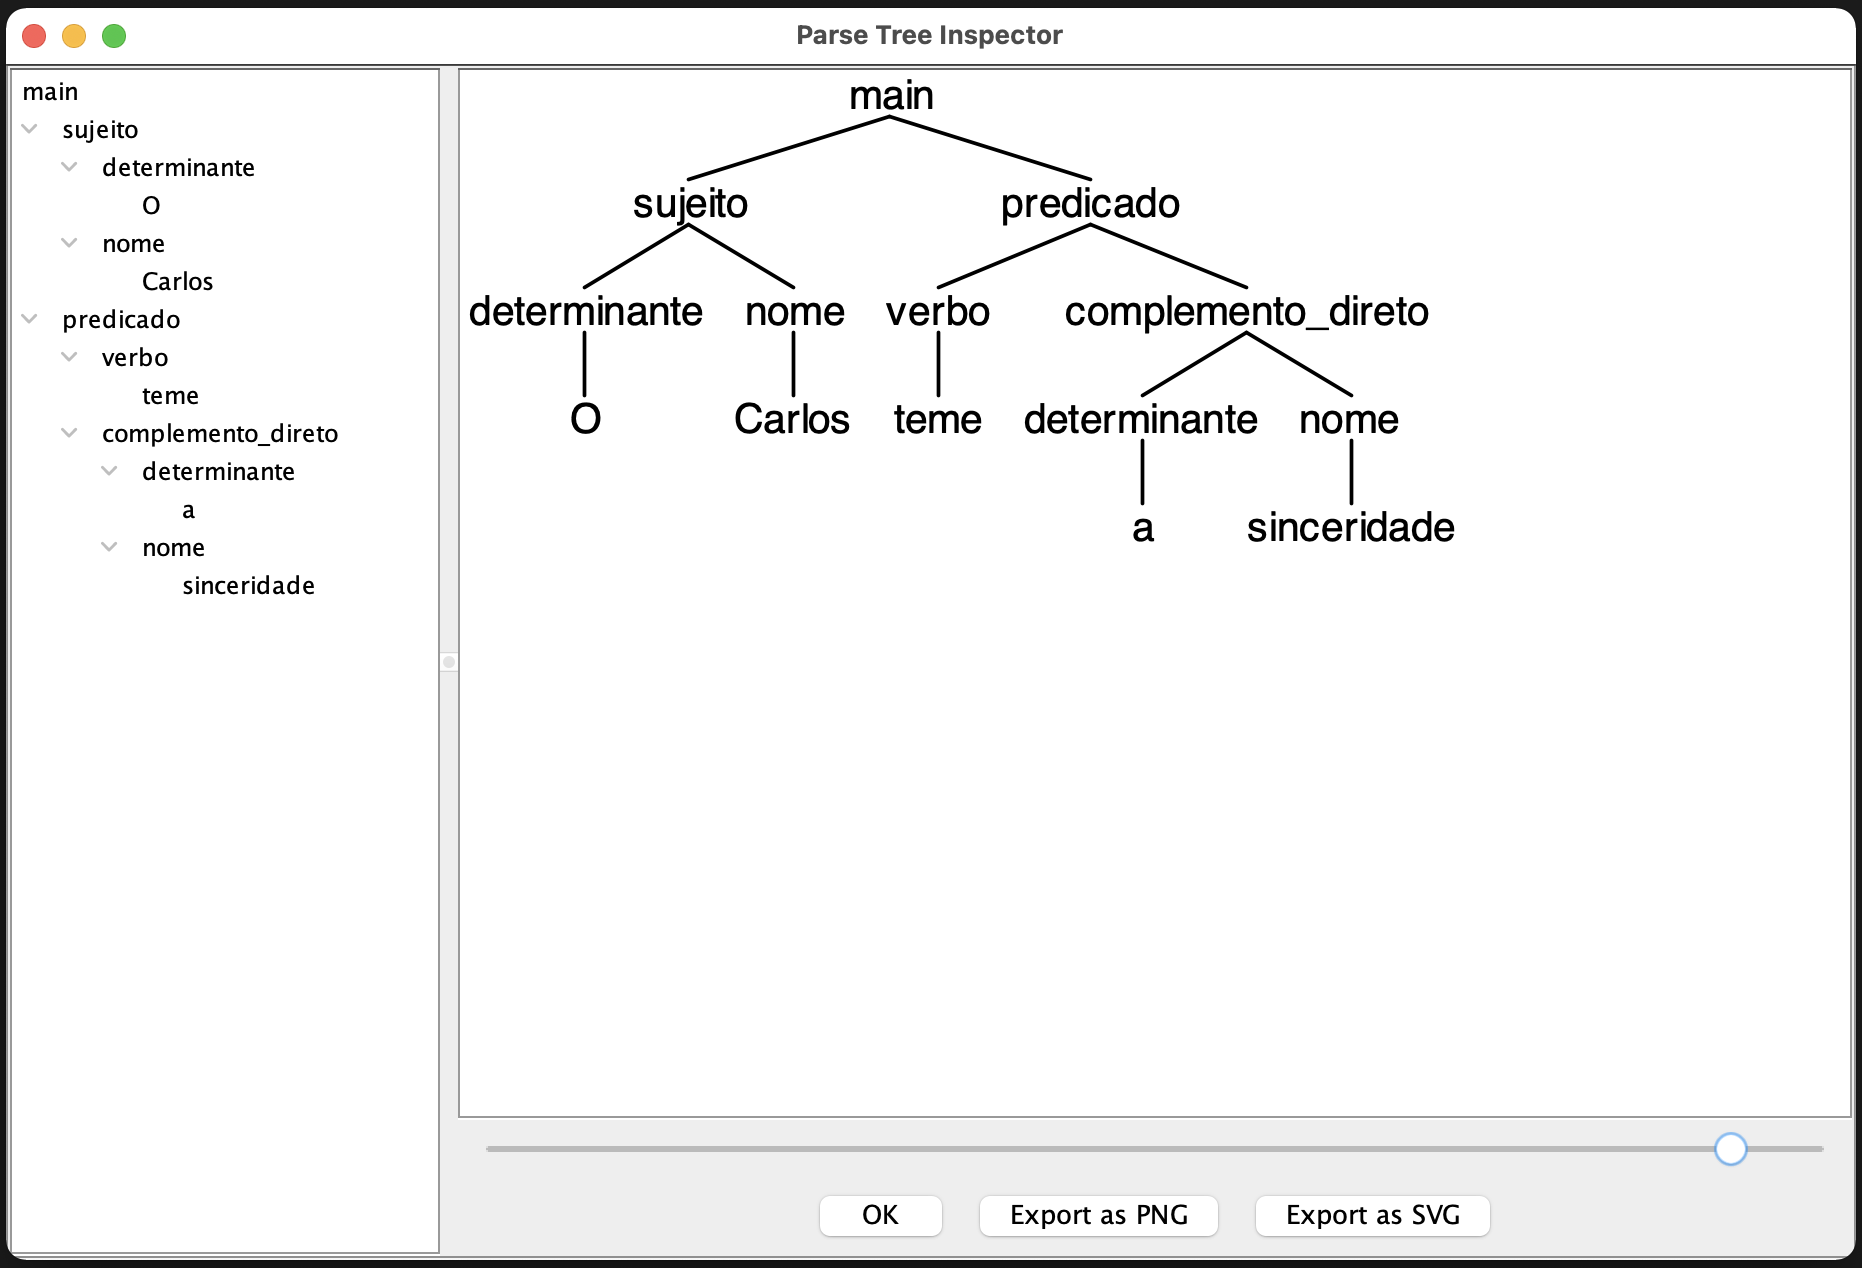
\includegraphics[width=10cm]{images/testrig_gui_example.png}
    \caption{Example of a generated syntax tree within TestRig.}
    \label{fig:system_architecture}
\end{figure}



% Having parsed the meta-language file, a generator is called by the main rule - the \emph{Rose Tree} is passed as an argument and then traversed in order to generate all 
% the rules for the Specific Natural Language Grammar.
% This grammar, after being generated, is used to create a processor in which the student's sentence will be used as input, creating a visual 
% syntax tree of that same sentence.
